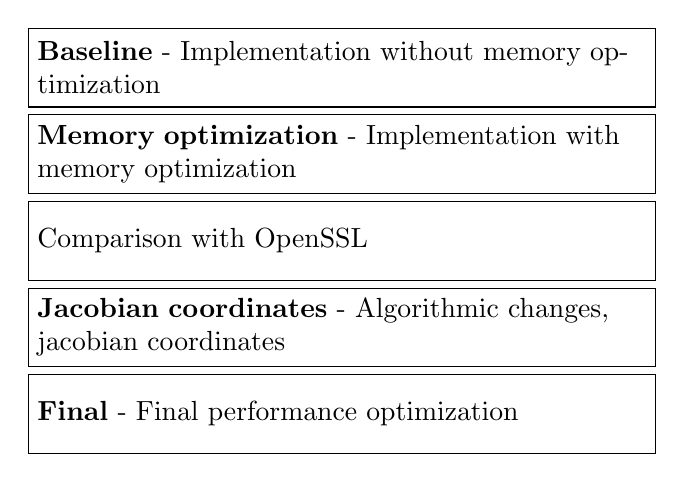
\begin{tikzpicture}[
rect/.style={
draw,
text width=22em,
minimum height = 1cm
},node distance=1.1cm
]
\node[rect] (1) {\textbf{Baseline} - Implementation without memory optimization};
\node[rect, below of=1] (2) {\textbf{Memory optimization} - Implementation with memory optimization};
\node[rect, below of=2] (3) {Comparison with OpenSSL};
\node[rect, below of=3] (4) {\textbf{Jacobian coordinates} - Algorithmic changes, jacobian coordinates};
\node[rect, below of=4] (5) {\textbf{Final} - Final performance optimization };

\end{tikzpicture}